\documentclass[10pt]{amsart}
\usepackage[margin=1in]{geometry}
\usepackage{amsmath,amssymb,amsthm}

\usepackage{graphicx}
\usepackage{pstricks}
\usepackage{pst-plot}
\usepackage{wrapfig}
\usepackage{multicol}
\usepackage{hyperref}

\usepackage{fancyhdr}
\pagestyle{fancyplain}
\usepackage{lastpage}

\newcommand{\mytitle}{Application Problems}
\newcommand{\myclass}{Math 341}

\rhead{pg. \thepage  \ of \pageref{LastPage}}    
\chead{\myclass}
\lhead{\mytitle}
\lfoot{\noindent(Draft \today)}
\cfoot{}


%The purpose of this code is to allow me to put lines in matrices so that I can create augmented matrices.
\makeatletter
\renewcommand*\env@matrix[1][*\c@MaxMatrixCols c]{%
  \hskip -\arraycolsep
  \let\@ifnextchar\new@ifnextchar
  \array{#1}}
\makeatother



\newcommand{\ds}{\displaystyle}
\begin{document}

\noindent{\huge{\bf \mytitle}}
\begin{multicols}{2}
\begin{enumerate}
\item[I] In each of the following scenarios, find a polynomial of least degree which passes through the given points. Then plot the points and the polynomial.
\item $(1,2),(3,3)$ 			
\item $(0,1),(2,3),(-1,4)$  
\item $(1,1),(2,2),(-1,5)$   
\item $(1,2),(3,3),(5,6)$ 			
\item $(1,2),(3,3),(5,5)$ 
\item $(0,1),(1,3),(-1,4),(2,4)$ 



\vspace{.3in}
\item[II] Compute each integral by finding a partial fraction decomposition. The form of the decomposition is provided.
\item $\ds\int\frac{1}{(x-3)(x+2)}dx , \frac{A}{x-3}+\frac{B}{x+2}$         
\item $\ds\int\frac{2x+3}{(x-3)(x+2)}dx, \frac{A}{x-3}+\frac{B}{x+2}$ 
\item $\ds\int\frac{x}{(x+1)(x-2)}dx,  \frac{A}{x+1}+\frac{B}{x-2}$  
\item $\ds\int\frac{x^2+2}{x^2(x-2)}dx, \frac{A}{x}+\frac{B}{x^2}+\frac{C}{x-2}$ 
\item $\ds\int\frac{1}{(x^2+1)(x-2)}dx, \frac{Ax+B}{x^2+1}+\frac{C}{x-2}$
\item $\ds\int\frac{x+1}{(x^2+1)x^2}dx, \frac{Ax+B}{x^2+1}+\frac{C}{x}+\frac{D}{x^2}$  




\vspace{.3in}
\item[III] Consider the following electrical system. Use the given values to find the current in each wire.

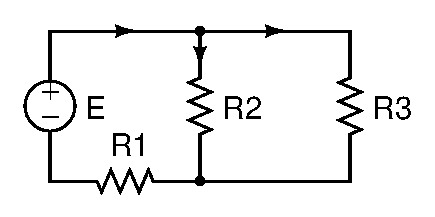
\includegraphics[height=.7in]{electric-circuit-hw1}

\item $E=12, R_1=2,R_2=2, R_3=2$.
\item $E=12, R_1=2,R_2=3, R_3=3$.
\item $E=12, R_1=2,R_2=3, R_3=6$.
\item $E=12, R_1=1,R_2=2, R_3=2$.
\item $E=9, R_1=3,R_2=1, R_3=2$.
\item $E=6, R_1=1,R_2=1, R_3=2$.



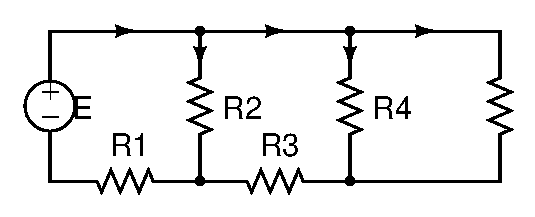
\includegraphics[height=.7in]{electric-circuit-hw2}

Use the 3 loop network above to setup an augmented matrix whose reduced form will give the currents in each wire.  Then use software to find the currents.
\item $E=12, R_1=2,R_2=2,R_3=3, R_4=6,R_5=1$
\item $E=120, R_1=2,R_2=10,R_3=3, R_4=6,R_5=4$


\vspace{.3in}
\item[IV] Find the derivative (as a matrix) of each function.
\item $f(x,y)=4x-3y^2$
\item $f(x,y)=4xy-3y^2$
\item $f(x,y,z)=x^2+2xy-3y^2+z$
\item $f(x,y,z)=2xy^3+3yz^2$
\item $\vec r(t)=\left<t^3, \sin(2t)\right>$
\item $\vec r(t)=\left<2t+1, 7, -2t\right>$
\item $\vec T(u,v)=\left<u+v, u-v\right>$
\item $\vec r(u,v)=\left<uv,2u+v, u^2-v^3\right>$






\vspace{.3in}
\item[V] Use differentials to make appropriate approximations in the following problems.

\item The dimensions of a rectangular box are supposed to be 2 by 3 by 5 feet. Use differentials to estimate the change in the volume of the box if 2 increase to 2.1, 3 increase to 3.2, and 5 decreases to 4.7 inches? 
\item The radius of a cylindrical metal disc (similar to a washer) is supposed to be 2 inches, with height .1 inches. The manufacturing process used to make this disc is not perfect and sometimes creates discs which are 2.05 inches in radius, and .11 inches in height (so $dr$ = .05 and $dh$=.01). The volume of a cylinder is $V=\pi r^2 h$. Use differentials to estimate how much this manufacturing imperfection will increase the volume of one metal disc? If a manufacturer needs to create 100 million of these discs for worldwide shipments, how much additional metal is needed because of this manufacturing imperfection? 
\item A right triangle is to be made with side lengths 3 and 4 inches.  By about how much will the length of the hypotenuse change if the side lengths change from 3 to 3.1 and 4 to 4.2 inches? 
\item An object moves in the plane approximately following the curve $x=2t+1 , y=t^2-1$ (meaning you have a function $r(t)=\left<2t+1,t^2-1\right>$.  By about how much will $x$ and $y$ change from $t=1$ to $t=1.2$? (This idea generalizes to give tangent lines to curves in space, something you would study in multivariable calculus.)






\vspace{.3in}
\item[VI] For each function, find the location of all critical points. Then use the second derivative test to determine if each critical point corresponds to a maximum, minimum, or saddle point. Graph the function in 3D to verify your results, and locate the eigenvectors and eigenvalues in the picture.
\item $f(x,y) = x^2+xy+y^2$
\item $f(x,y) = x^2+4xy+y^2$
\item $f(x,y) = x^2+2xy+y^2$
\item $f(x,y) = x^2-4x+y^2+2y+1$
\item $f(x,y) = x^2-2x+xy+y^2$
\item $f(x,y) = x^2+xy+3y^2$
\item $f(x,y) = x^3-3x+y^2-2y$ (2 critical points)
\item $f(x,y) = x^3-3x+y^3-3y^2$ (4 critical points)





\vspace{.3in}
\item[VII] Markov Process - In each scenario, write the transition matrix. If an initial state is given, then find the next two states. Finish by finding a steady state solution and use it to answer the question at the end.

\item In a certain town, there are 3 types of land zones: residential, commercial, and industrial. The city has been undergoing growth recently, and the city has noticed the following trends.  Every 5 years, 10\% of the older residential land gets rezoned as commercial land, while 5\% gets rezoned as industrial.  The other 85\% remains residential.  For commercial land, 70\% remains commercial, while 10\% becomes residential and 20\% becomes industrial. For industrial land, 60\% remains industrial, while 25\% becomes commercial and 15\% becomes residential. Currently the percent of land in each zone is 40\% residential, 30\% commercial, and 30\% industrial. What will the percent distribution be in 5 years? In 10 years?  If this trend continues indefinitely, what percent of the land will eventually be residential?. (Solution: the ratios are 4:3:2, so 4/9 will be residential, or 44.4\%)
\item Suppose we own a car rental company which rents cars in Idaho Falls and Rexburg. The last few weeks have shown a weekly trend that 60\% of the cars rented in Rexburg will remain in Rexburg (the other 40\% end up in IF), whereas 80\% of the cars rented in Idaho Falls will remain in Idaho Falls. If there are currently 60 cars in Rexburg and 140 cars in IF, how many will be in each city next week?  In two weeks? In three weeks? If this trend continues indefinitely, about how many cars should you expect to find in Rexburg each week?
\item Repeat the previous problem if 40\% of the cars rented in Rexburg will remain in Rexburg (the other 60\% end up in IF), whereas 80\% of the cars rented in Idaho Falls will remain in Idaho Falls.
\item Repeat the previous problem if 70\% of the cars rented in Rexburg will remain in Rexburg (the other 30\% end up in IF), whereas 80\% of the cars rented in Idaho Falls will remain in Idaho Falls.
\item A school cafeteria regularly offers 3 types of meals to its students. One of the meals is always a pizza/salad combo, One is always hamburgers and fries, and one is a daily special which changes daily. In an attempt to understand student preferences, the school discovered the following information. If a student has a hamburger one day, then there is a 30\% chance they will try the daily special the next day, and a 40\% percent chance they will have the salad bar.  If they have the salad bar, then there is a 30\% chance they'll switch to the daily special, and a 40\% chance they'll switch to the hamburger.  If the have the daily special, then there is a 50\% chance they'll get the daily special the next day, a 20\% chance they'll switch to pizza, and a 30\% chance they'll switch to hamburger.  If this trend continues, what percent of the students will eat each type of meal? 

[While this problem is highly rigged, there is a branch of applied mathematics which is studied by financial analysts call stochastic processes which models such a scenario. This modeling process can help predict how a new restaurant will perform in a city, sometimes predict stock market fluctuations, and more. The study of stochastic processes begins with a Markov process and then introduces statistics and probability to help predict what happens when trends change.]





\vspace{.3in}
\item[VIII] For each matrix, find a basis for the column and row space by writing the matrix in the form $A=CR$. Write each column and row of the matrix as a linear combination of these basis vectors. If the row or column space consists of 2D or 3D vectors, use the computer to draw the vector space, where your basis vectors give the grid lines to follow in your illustration. This section is pattern recognition. Once you see the pattern, try it on one a larger matrix and then move on.


\item $\begin{bmatrix} 1&2\\0&3 \end{bmatrix}$
\item $\begin{bmatrix} 2&4\\2&1 \end{bmatrix}$
\item $\begin{bmatrix} 0&1\\0&3 \end{bmatrix}$
\item $\begin{bmatrix} 1&0&2\\0&1&-1\\0&1&-1 \end{bmatrix}$
\item $\begin{bmatrix} 0&0&2\\1&2&0\\-1&-2&1 \end{bmatrix}$

\item $\begin{bmatrix} 0&1&2\\1&3&-1 \end{bmatrix}$
\item $\begin{bmatrix} 0&1\\0&3\\2&0 \end{bmatrix}$

\item $\begin{bmatrix} 0&0&2&-2\\1&2&0&2\\-1&-2&1&-3 \end{bmatrix}$


\vspace{.3in}
\item[IX] For each set of data points, find an equation of the least squares regression line. Plot the points and the line on the same axes.

\item $(0,0),(1,3),(1,2)$
\item $(1,1),(2,1),(3,2)$
\item $(1,2),(3,0),(5,1)$
\item $(0,0),(1,3),(1,2),(4,5)$
\item $(0,0),(1,3),(1,2),(4,-5)$
\item $(-1,2),(1,3),(2,5),(3,3)$
\item Challenge: Find an equation of the least squares regression parabola $y=ax^2+bx+c$ which passes through the points $(0,0),(1,3),(1,2),(4,5)$. [Hint, you will need a 4 by 3 matrix for $A$ instead of an $n$ by $2$. Use the transpose to reduce the size of the matrix to a 3 by 3 matrix, and then solve.]


\vspace{.3in}
\item[X] Use Cramer's rule to find solutions to the following linear systems. If Cramer's rule fails, explain why.

\item $2x+3y=0, x-2y=1$
\item $x+y=2, x-y=3$
\item $3x+y=6, x+3y=2$
\item $2x+y=1, 4x+2y=2$
\item $x+y=0, 2x-y+z=1, x+z=0$
\item $x+2y=3, x-y+z=0, x+3y+z=1$
\item $y+2z=1, x-z=3, 2x+y=1$



\end{enumerate}









%\newpage
\small
Solutions: Remember that the Technology introduction has a step-by-step guide for solving many of these problems.
\begin{enumerate}

\item[I] Interpolating Polynomials
\item $1/2 x + 3/2$
\item $(4/3)x^2-(5/3)x+1$
\item $x^2-2x+2$
\item $(1/4)x^2-(1/2)x+9/4$
\item $(1/8)x^2+15/8$
\item $-x^3+(5/2)x^2+(1/2)x+1$




\item[II] Partial Fractions
\item $-1/5\,\ln  \left( x+2 \right) +1/5\,\ln  \left( x-3 \right)$
\item $1/5\,\ln  \left( x+2 \right) +9/5\,\ln  \left( x-3 \right) $
\item $1/3\,\ln  \left( x+1 \right) +2/3\,\ln  \left( x-2 \right) $
\item ${x}^{-1}+3/2\,\ln  \left( x-2 \right) -1/2\,\ln  \left( x \right)$
\item $-\frac{1}{10}\ln  \left( {x}^{2}+1 \right) -\frac{2}{5}\arctan \left( x \right) +\frac{1}{5}\ln  \left( x-2 \right) $
\item $-{x}^{-1}-1/2\,\ln  \left( {x}^{2}+1 \right) -\arctan \left( x
 \right) +\ln  \left( x \right)
$



\item[III] Kirchoff's Laws

 $\begin{bmatrix}[lll|l]
 1 & -1 & -1 & 0 \\
 R_1 & R_2 & 0 & E \\
 0 & -R_2 & R_3 & 0
\end{bmatrix}$

\item $(4,2,2)$
\item $(24/7,12/7,12/7)$
\item $(3,2,1)$
\item $(6,3,3)$
\item $(27/11,18/11,9/11)$
\item $(18/5,12/5,6/5)$

$\begin{bmatrix}[llllll|l]
 1 & -1 & -1 & 0 & 0 & 0 & 0 \\
 0 & 0 & 1 & -1 & -1 & 0 & 0 \\
 0 & 0 & 0 & 1 & 1 & -1 & 0 \\
 R_1 & R_2 & 0 & 0 & 0 & 0 & E \\
 0 & -R_2 & 0 & R_4 & 0 & R_3 & 0 \\
 0 & 0 & 0 & -R_4 & R_5 & 0 & 0
\end{bmatrix}$

\item $\left(\frac{123}{34},\frac{81}{34},\frac{21}{17},\frac{3}{17},\frac{18}{17},\frac{21}{17}\right)$

\item $\left(\frac{231}{106},\frac{81}{106},\frac{75}{53},\frac{30}{53},\frac{45}{53},\frac{75}{53}\right)$

\item[IV] Derivatives

\item $\begin{bmatrix}4 & -6y\end{bmatrix}$
\item $\begin{bmatrix}4y & -6y\end{bmatrix}$
\item $\begin{bmatrix}2x+2y & 2x-6y & 1\end{bmatrix}$
\item $\begin{bmatrix}2y^3 & 6xy^2+3z^2 & 6yz\end{bmatrix}$
\item $\begin{bmatrix}3t^2\\ 2\cos(2t)\end{bmatrix}$
\item $\begin{bmatrix}2\\0\\-2\end{bmatrix}$
\item $\begin{bmatrix}1&1\\1&-1\end{bmatrix}$
\item $\begin{bmatrix}v&u\\2&1\\2u&-3v^2\end{bmatrix}$


\item[V]Approximation
\item $1.7$
\item $.188496$
\item $.022$
\item $dx=.4,dy=.4$


\item[VI] Second Derivative Test
\item At $(0,0)$ eigenvalues are $3,1$ (both positive so min) with eigenvectors $[1,1]^T,[-1,1]^T$.
\item At $(0,0)$ eigenvalues are $6,-2$ (saddle point) with eigenvectors $[1,1]^T,[-1,1]^T$.
\item At $(0,0)$ eigenvalues are $4,0$ (test fails) with eigenvectors $[1,1]^T,[-1,1]^T$.
\item At $(2,-1)$ eigenvalues are $2,2$ (both positive so min) with eigenvectors $[1,0]^T,[0,1]^T$.
\item At $(4/3,-2/3)$ eigenvalues are $3,1$ (both positive so min) with eigenvectors $[1,1]^T,[-1,1]^T$.
\item At $(0,0)$ eigenvalues are $6.23607,1.76393$ (both positive so min) with eigenvectors $[.236,1]^T,[-4.236,1]^T$.
\item 
At $(-1,1)$ eigenvalues are $-6,2$ (saddle) with eigenvectors $[1,0]^T,[0,1]^T$.
At $(1,1)$ eigenvalues are $6,2$ (both positive so min) with eigenvectors $[1,0]^T,[0,1]^T$.
\item 
At $(-1,0)$ eigenvalues are $-6,-6$ (both negative so max) with eigenvectors $[1,0]^T,[0,1]^T$.
At $(-1,2)$ eigenvalues are $-6,6$ (saddle) with eigenvectors $[1,0]^T,[0,1]^T$.
At $(1,0)$ eigenvalues are $6,-6$ (saddle) with eigenvectors $[1,0]^T,[0,1]^T$.
At $(1,2)$ eigenvalues are $6,6$ (both positive so min) with eigenvectors $[1,0]^T,[0,1]^T$.







\item[VII] Markov Process

\item Transition matrix 
$\begin{bmatrix}
 0.85 & 0.1 & 0.15 \\
 0.1 & 0.7 & 0.25 \\
 0.05 & 0.2 & 0.6
\end{bmatrix}$,
5 years  (41.5,32.5,26), 
10 years: (42.425,33.4,24.175),
Steady state: $[4,3,2]^T$ so 4/9 or 44.4\% will be residential. 

\item
Transition matrix 
$\begin{bmatrix}
 {3}/{5} & {1}/{5} \\
 {2}/{5} & {4}/{5}
\end{bmatrix}$,
1 week  (64,136), 
2 week: (65.6,134.4),
3 week: (66.24,133.76),
Steady state: $[1,2]^T$ so 1/3 (33.3\%) will be in Rexburg. This means 66 or 67 cars will be in Rexburg. 
 
\item 
Transition matrix 
$\begin{bmatrix}
 {2}/{5} & {1}/{5} \\
 {3}/{5} & {4}/{5}
\end{bmatrix}$,
1 week  (52,148), 
2 week: (50.4,149.6),
3 week: (50.08,149.92),
Steady state: $[1,3]^T$ so 1/4 or 25\% will be in Rexburg. This means 50 cars will be in Rexburg. 

\item 
Transition matrix 
$\begin{bmatrix}
 {7}/{10} & {1}/{5} \\
 {3}/{10} & {4}/{5}
\end{bmatrix}$,
1 week  (70,130), 
2 week: (75,125),
3 week: (77.5,122.5),
Steady state: $[2,3]^T$ so 2/5 or 40\% will be in Rexburg. This means 80 cars will be in Rexburg. 

\item My order is hamburger, pizza/salad, special (your order may vary which means your matrix will be a little different, but the eigenvector will still have the same ratios).
Transition matrix 
$\begin{bmatrix}
 {3}/{10} & {2}/{5} & {3}/{10} \\
 {2}/{5} & {3}/{10} & {1}/{5} \\
 {3}/{10} & {3}/{10} & {1}/{2}
\end{bmatrix}$,
Steady state: $[29,26,33]^T$ or $[29/88,26/88,33/88]^T$ so Hamburger - 32.9545\%, Pizza/Salad - 29.5455\%, Special - 37.5\%. 















%
%\vspace{.3in}
\item[VIII] Column and Row Space ---- Notice in all of the problems below that each column is a linear combination of the pivot columns, using the columns of RREF as the coefficients.  Also notice that each row is a linear combination of the rows of RREF, using the columns of the original matrix as the coefficients.
%For each matrix, find a basis for the column and row space by writing the matrix in the form $A=CR$. Write each column and row of the matrix as a linear combination of these basis vectors. If the row or column space consists of 2D or 3D vectors, use the computer to draw the vector space, where your basis vectors give the grid lines to follow in your illustration. This section is pattern recognition. Once you see the pattern, try it on one a larger matrix and then move on.
%
%
\item 
$A=\begin{bmatrix} 1&2\\0&3 \end{bmatrix}\begin{bmatrix} 1&0\\0&1 \end{bmatrix}, 
\begin{bmatrix} 1\\0 \end{bmatrix}=1\begin{bmatrix} 1\\0 \end{bmatrix}+0\begin{bmatrix} 2\\3 \end{bmatrix},
\begin{bmatrix} 2\\3 \end{bmatrix}=0\begin{bmatrix} 1\\0 \end{bmatrix}+1\begin{bmatrix} 2\\3 \end{bmatrix},
\begin{bmatrix} 1&2 \end{bmatrix}=1\begin{bmatrix} 1&0 \end{bmatrix}+2\begin{bmatrix} 0&1 \end{bmatrix},
\begin{bmatrix} 0&3 \end{bmatrix}=0\begin{bmatrix} 1&0 \end{bmatrix}+3\begin{bmatrix} 0&1 \end{bmatrix}.
$

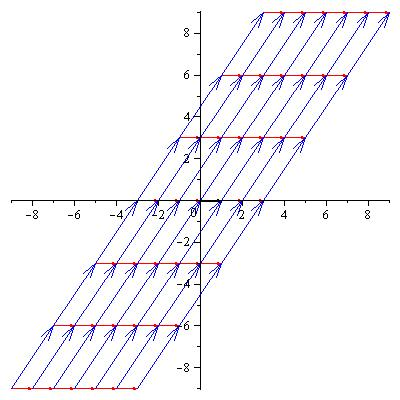
\includegraphics[height=1in]{support/vs1}
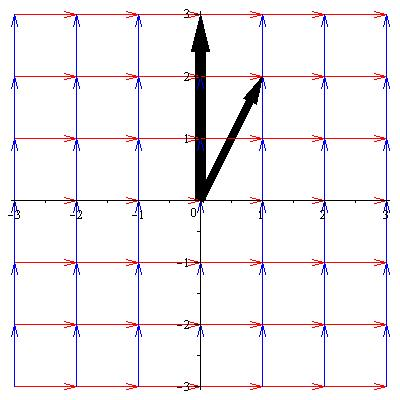
\includegraphics[height=1in]{support/vsr1}
%$\begin{bmatrix} 1&2\\0&3 \end{bmatrix}$

\item 
$A=\begin{bmatrix} 2&4\\2&1 \end{bmatrix}\begin{bmatrix} 1&0\\0&1 \end{bmatrix},
\begin{bmatrix} 2\\2 \end{bmatrix}=1\begin{bmatrix} 2\\2 \end{bmatrix}+0\begin{bmatrix} 4\\1 \end{bmatrix},
\begin{bmatrix} 4\\1 \end{bmatrix}=0\begin{bmatrix} 2\\2 \end{bmatrix}+1\begin{bmatrix} 4\\1 \end{bmatrix},
\begin{bmatrix} 2&4 \end{bmatrix}=2\begin{bmatrix} 1&0 \end{bmatrix}+4\begin{bmatrix} 0&1 \end{bmatrix},
\begin{bmatrix} 2&1 \end{bmatrix}=2\begin{bmatrix} 1&0 \end{bmatrix}+1\begin{bmatrix} 0&1 \end{bmatrix},
$

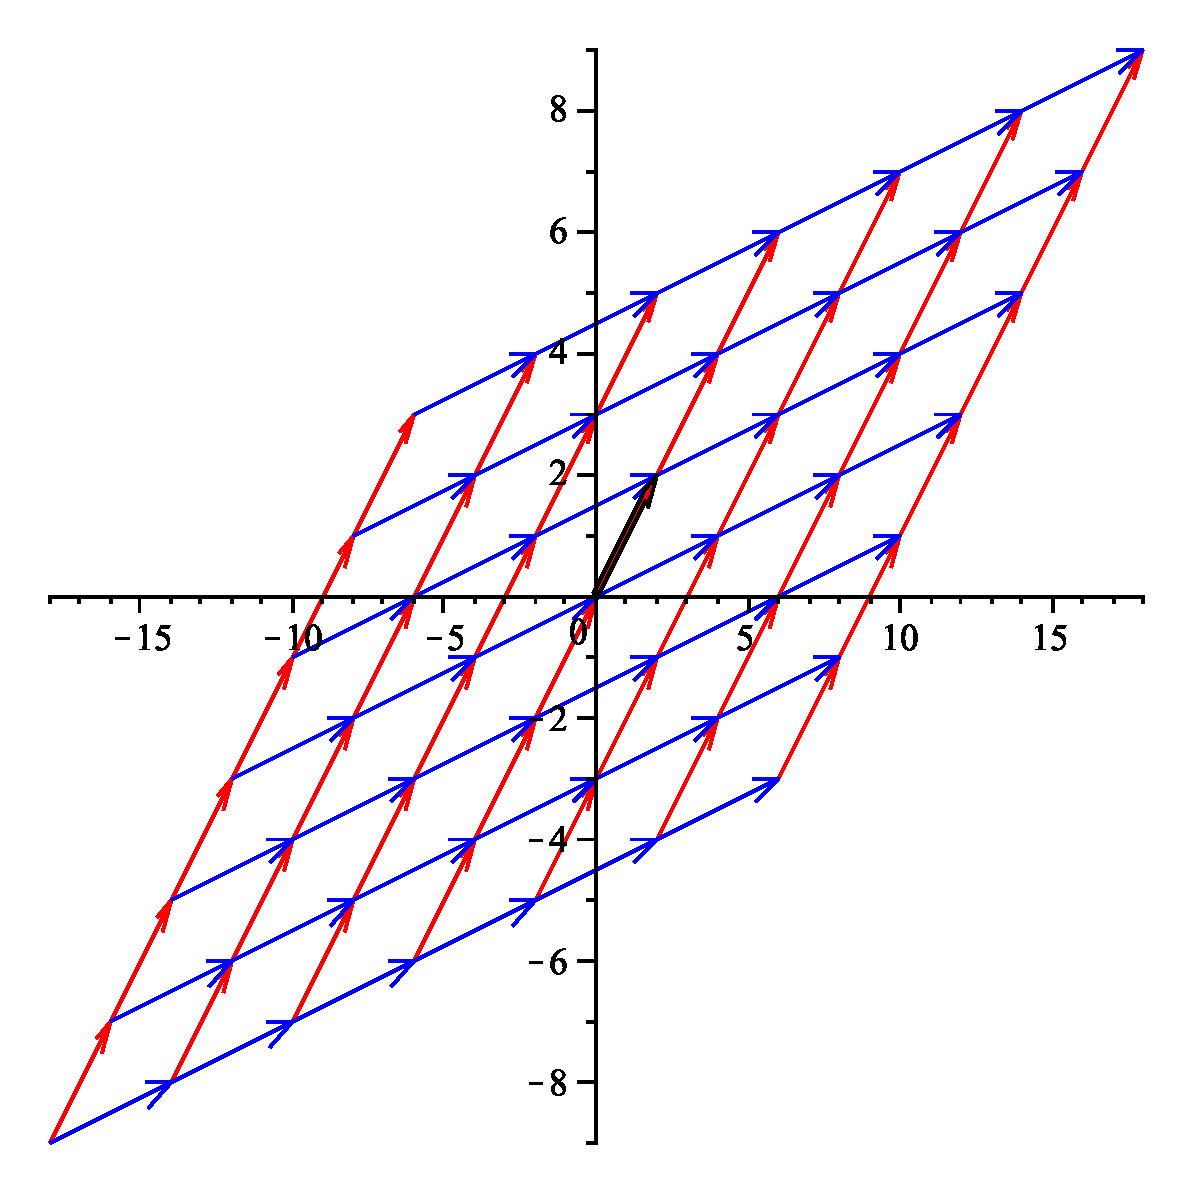
\includegraphics[height=1in]{support/vs2}
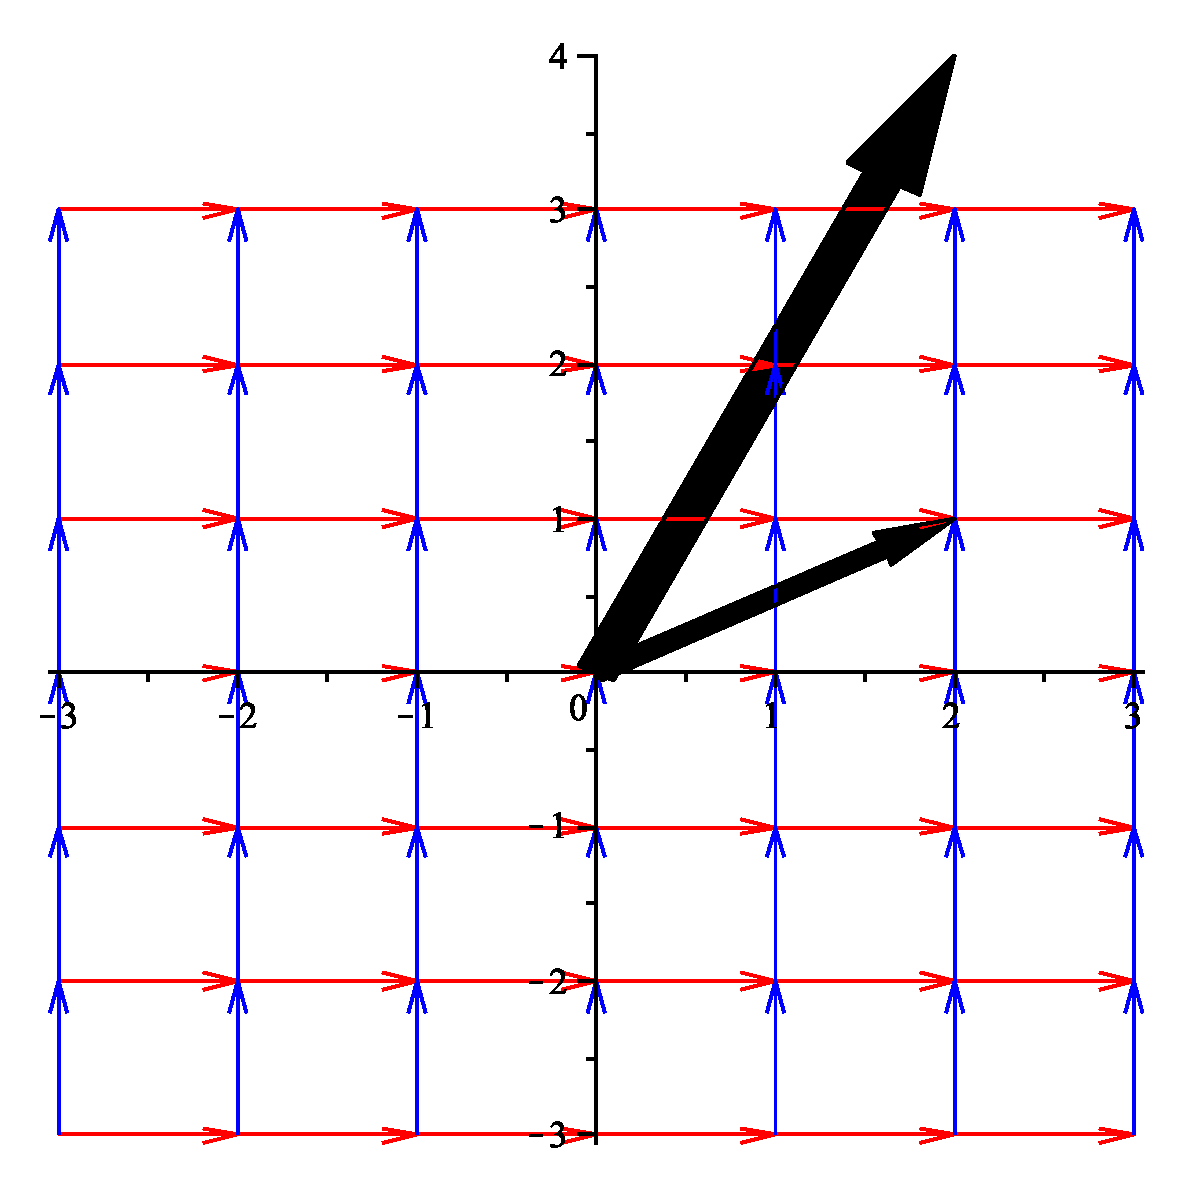
\includegraphics[height=1in]{support/vsr2}

%$\begin{bmatrix} 2&4\\2&1 \end{bmatrix}$

\item 
$A=\begin{bmatrix} 1\\3 \end{bmatrix}\begin{bmatrix} 0&1 \end{bmatrix},
\begin{bmatrix} 0\\0 \end{bmatrix}=0\begin{bmatrix} 1\\3 \end{bmatrix},
\begin{bmatrix} 1\\3 \end{bmatrix}=1\begin{bmatrix} 1\\3 \end{bmatrix},
\begin{bmatrix} 0&1 \end{bmatrix}=1\begin{bmatrix} 0&1 \end{bmatrix},
\begin{bmatrix} 0&3 \end{bmatrix}=3\begin{bmatrix} 0&1 \end{bmatrix},
$

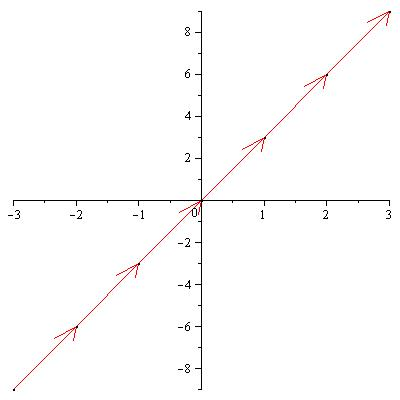
\includegraphics[height=1in]{support/vs3}
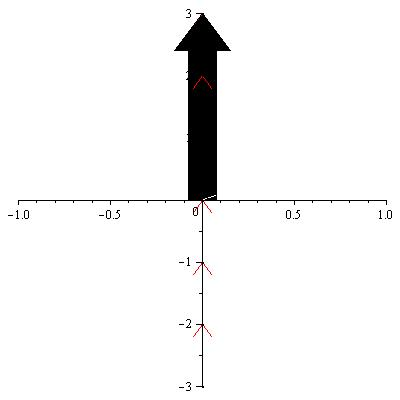
\includegraphics[height=1in]{support/vsr3}

%$\begin{bmatrix} 0&1\\0&3 \end{bmatrix}$


\item 
$A=\begin{bmatrix} 1&0\\0&1\\0&1 \end{bmatrix}\begin{bmatrix} 1&0&2\\0&1&-1 \end{bmatrix},
\begin{bmatrix} 1\\0\\0 \end{bmatrix} = 1\begin{bmatrix} 1\\0\\0 \end{bmatrix}+0\begin{bmatrix} 0\\1\\1 \end{bmatrix},
\begin{bmatrix} 0\\1\\1 \end{bmatrix} = 0\begin{bmatrix} 1\\0\\0 \end{bmatrix}+1\begin{bmatrix} 0\\1\\1 \end{bmatrix},
\begin{bmatrix} 2\\-1\\-1 \end{bmatrix} = 2\begin{bmatrix} 1\\0\\0 \end{bmatrix}-1\begin{bmatrix} 0\\1\\1 \end{bmatrix},
\begin{bmatrix} 1&0&2 \end{bmatrix}=1\begin{bmatrix} 1&0&2 \end{bmatrix}+0\begin{bmatrix} 0&1&-1 \end{bmatrix},
\begin{bmatrix} 0&1&-1 \end{bmatrix}=0\begin{bmatrix} 1&0&2 \end{bmatrix}+1\begin{bmatrix} 0&1&-1 \end{bmatrix},
$

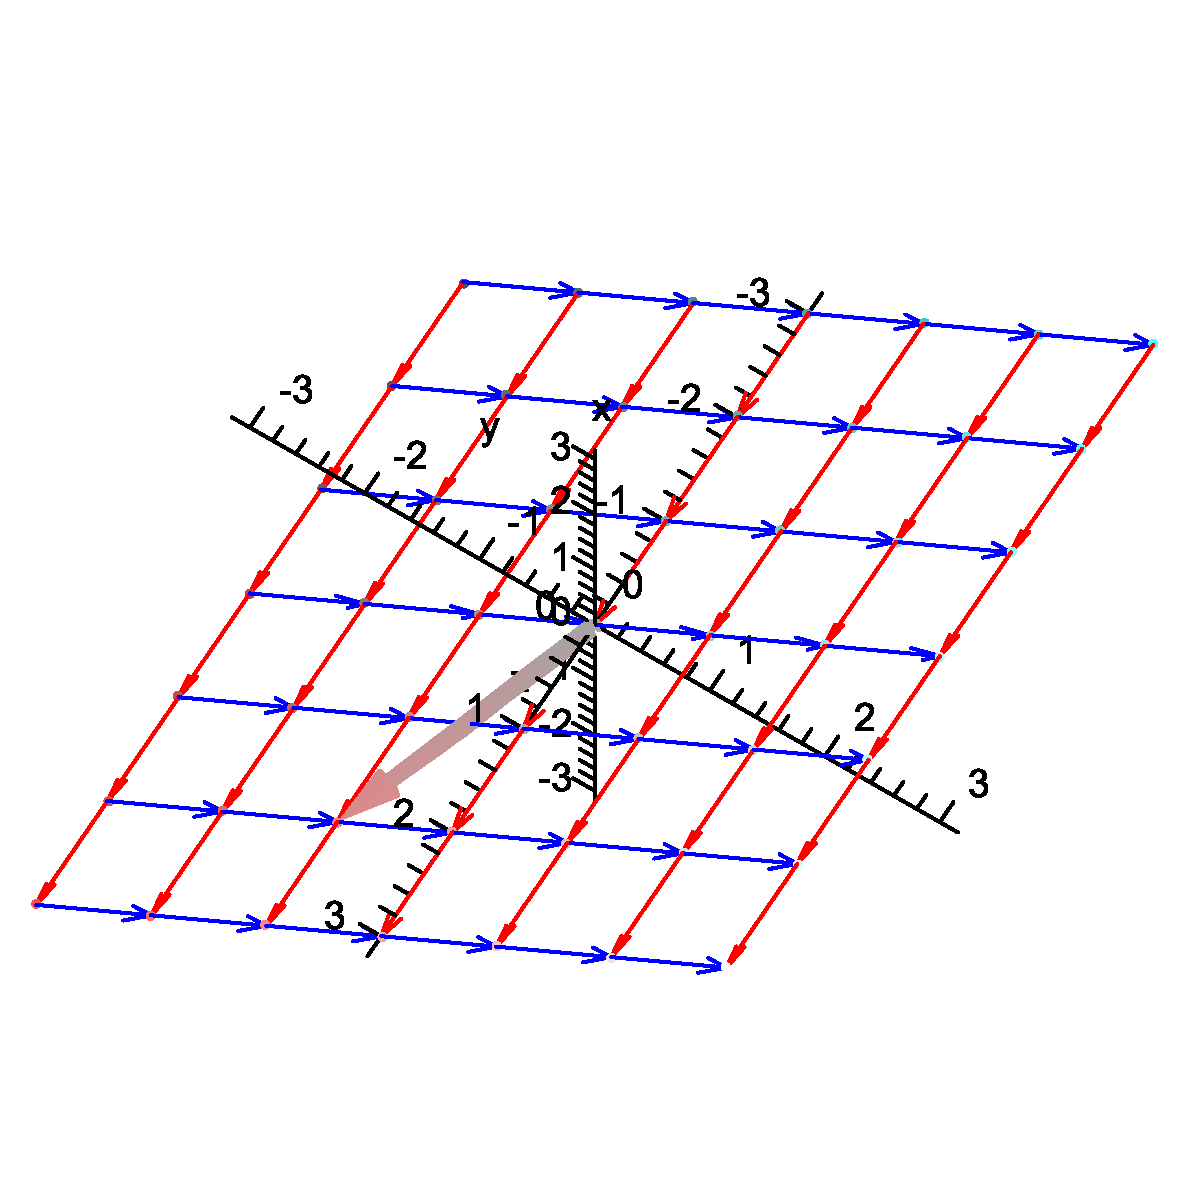
\includegraphics[height=1in]{support/vs4}
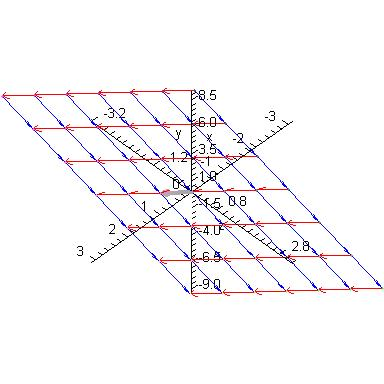
\includegraphics[height=1in]{support/vsr4}

%$\begin{bmatrix} 1&0&2\\0&1&-1\\0&1&-1 \end{bmatrix}$


\item 
$A=\begin{bmatrix} 0&2\\1&0\\-1&1 \end{bmatrix}\begin{bmatrix} 1&2&0\\0&0&1 \end{bmatrix},
\begin{bmatrix} 0\\1\\-1 \end{bmatrix} = 1\begin{bmatrix} 0\\1\\-1 \end{bmatrix}+0\begin{bmatrix} 2\\0\\1 \end{bmatrix},
\begin{bmatrix} 0\\2\\-2 \end{bmatrix} = 2\begin{bmatrix} 0\\1\\-1 \end{bmatrix}+0\begin{bmatrix} 2\\0\\1 \end{bmatrix},
\begin{bmatrix} 2\\0\\1 \end{bmatrix} = 0\begin{bmatrix} 0\\1\\-1 \end{bmatrix}+1\begin{bmatrix} 2\\0\\1 \end{bmatrix},
\begin{bmatrix} 0&0&2 \end{bmatrix}=0\begin{bmatrix} 1&2&0 \end{bmatrix}+2\begin{bmatrix} 0&0&1 \end{bmatrix},
\begin{bmatrix} 1&2&0 \end{bmatrix}=1\begin{bmatrix} 1&2&0 \end{bmatrix}+0\begin{bmatrix} 0&0&1 \end{bmatrix},
\begin{bmatrix} -1&-2&1 \end{bmatrix}=-1\begin{bmatrix} 1&2&0 \end{bmatrix}+1\begin{bmatrix} 0&0&1 \end{bmatrix},
$

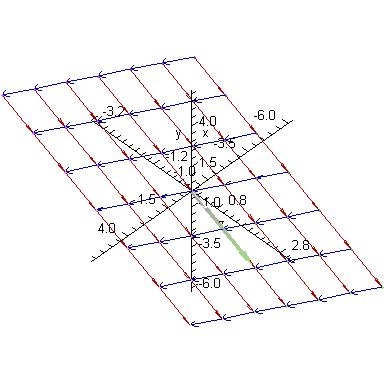
\includegraphics[height=1in]{support/vs5}
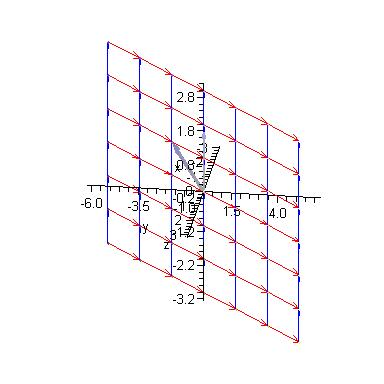
\includegraphics[height=1in]{support/vsr5}


%$\begin{bmatrix} 0&0&2\\1&2&0\\-1&-2&1 \end{bmatrix}$
%
\item 
%$\begin{bmatrix} 0&1&2\\1&3&-1 \end{bmatrix}$

\item 
%$\begin{bmatrix} 0&1\\0&3\\2&0 \end{bmatrix}$
%
\item 
%$\begin{bmatrix} 0&0&2&-2\\1&2&0&2\\-1&-2&1&-3 \end{bmatrix}$
%
%
%\vspace{.3in}
\item[IX] Regression (Make the plots using technology)
%For each set of data points, find an equation of the least squares regression line. Plot the points and the line on the same axes.

\item $y=\frac{5 x}{2}$
%$(0,0),(1,3),(1,2)$
\item $y=\frac{x}{2}+\frac{1}{3}$
%$(1,1),(2,1),(3,2)$
\item $y=\frac{7}{4}-\frac{x}{4}$
%$(1,2),(3,0),(5,1)$
\item $y=\frac{10 x}{9}+\frac{5}{6}$
%$(0,0),(1,3),(1,2),(4,5)$
\item $y=\frac{5}{2}-\frac{5 x}{3}$
%$(0,0),(1,3),(1,2),(4,-5)$
\item $y=\frac{3 x}{7}+\frac{19}{7}$
%$(-1,2),(1,3),(2,5),(3,3)$
\item 
$
A=
\begin{bmatrix} 
 0 & 0 & 1 \\
 1 & 1 & 1 \\
 1 & 1 & 1 \\
 16 & 4 & 1
\end{bmatrix},
B=
\begin{bmatrix} 
 0 \\
 3 \\
 2 \\
 5
\end{bmatrix},
A^T A=
\begin{bmatrix} 
 258 & 66 & 18 \\
 66 & 18 & 6 \\
 18 & 6 & 4
\end{bmatrix},
A^T B=
\begin{bmatrix} 
 85 \\
 25 \\
 10
\end{bmatrix}$,

$y=-\frac{5}{12}x^2+\frac{35}{12}x+0
$
%Challenge: Find an equation of the least squares regression parabola $y=ax^2+bx+c$ which passes through the points $(0,0),(1,3),(1,2),(4,5)$. [Hint, you will need a 4 by 3 matrix for $A$ instead of an $n$ by $2$. Use the transpose to reduce the size of the matrix to a 3 by 3 matrix, and then solve.]
%
%
%\vspace{.3in}
\item[X] Cramer's rule
%
\item $\left\{\frac{3}{7},-\frac{2}{7}\right\}$
%$2x+3y=0, x-2y=1$
\item $\left\{\frac{5}{2},-\frac{1}{2}\right\}$
%$x+y=2, x-y=3$
\item $\{2,0\}$
%$3x+y=6, x+3y=2$
\item Fails. The determinant of the coefficient matrix is zero.
%$2x+y=1, 4x+2y=2$
\item $\left\{\frac{1}{2},-\frac{1}{2},-\frac{1}{2}\right\}$
%$x+y=0, 2x-y+z=1, x+z=0$
\item $\left\{\frac{5}{2},\frac{1}{4},-\frac{9}{4}\right\}$
%$x+2y=3, x-y+z=0, x+3y+z=1$
\item Fails. The determinant of the coefficient matrix is zero.
%$y+2z=1, x-z=3, 2x+y=1$
%
%


















	
\end{enumerate}


\end{multicols}








\end{document}







